\chapter{Result and Discussion}
In this project, many low light images tested but only three images result kept in this report along with original images and enhanced images using different Retinex model, Power Law Transformation\cite{plt1}, Histogram Equalization\cite{he1} and Adaptive Histogram Equalization\cite{he2}. Also compared all these results with respect to Absolute Mean Difference(AMD),Root Mean Square \cite{amd1} and Entropy\cite{entropy}
\section{Retinex Model}
The main focus of this work is to enhance the low light images and this project is implemented in MATLAB tool. Figure \ref{fig:ssr} shows the original low light image of lamp and enhanced image using Single-Scale Retinex(SSR) model\cite{retinex}. It is clear enhancement in Figure \ref{fig:ssr}(b). The background objects of in figure \ref{fig:ssr}(b) are more clear than original image. The Absolute Mean Difference(AMD),Root Mean Square and Entropy for Single Scale Retinex(SSR) Model of enhanced image of lamp is $69.8401,15.7384$ and $4.9043$ respectively      



\begin{figure}[!htb]
	\begin{subfigure}{8cm}
		\centering    
    	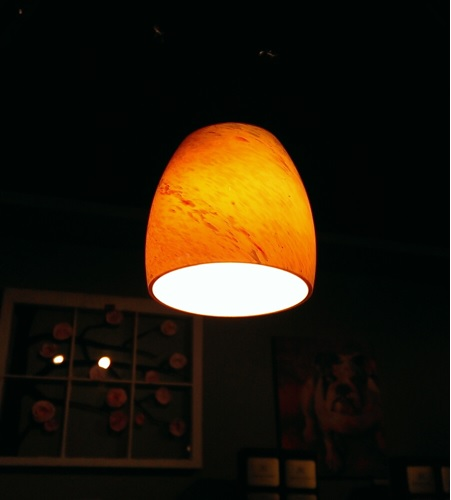
\includegraphics[width=7cm,height=9cm,keepaspectratio]{images/ch5/bulb_input.jpg}
    	\caption{} 
    \end{subfigure}
  	\begin{subfigure}{6cm}
  		\centering
  		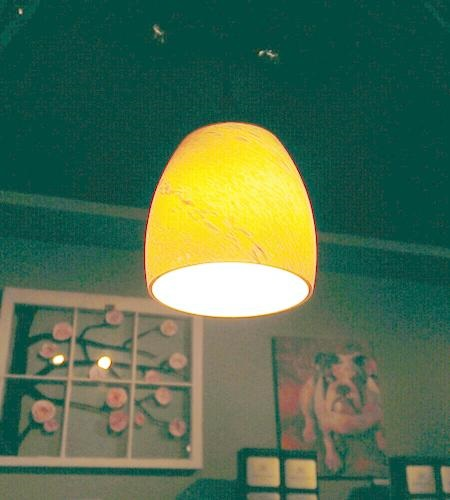
\includegraphics[width=7cm,height=9cm,keepaspectratio]{images/ch5/bulb_ssr.jpg}
   		\caption{}
  	\end{subfigure}
  	\caption{a) Input Image b)Enhanced Image using SSR}
  	\label{fig:ssr}
\end{figure}

Figure \ref{fig:msr} shows the original low light image of lamp and enhanced image using Multi-Scale Retinex(MSR) model. It is clear enhancement in Figure \ref{fig:msr}(b). The background objects of in figure \ref{fig:msr}(b) are more clear than original image. The Absolute Mean Difference(AMD),Root Mean Square and Entropy for Multi-Scale Retinex(MSR) model of enhanced image of lamp is $69.9617, 15.7384$ and $5.0033$ respectively      


\begin{figure}[!htb]
	\begin{subfigure}{8cm}
		\centering    
    	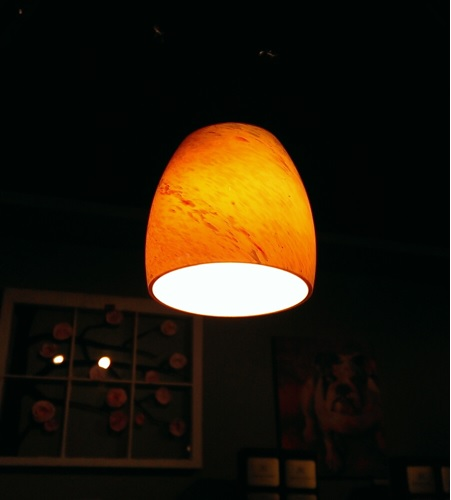
\includegraphics[width=7cm,height=9cm,keepaspectratio]{images/ch5/bulb_input.jpg}
    	\caption{} 
    \end{subfigure}
  	\begin{subfigure}{6cm}
  		\centering
  		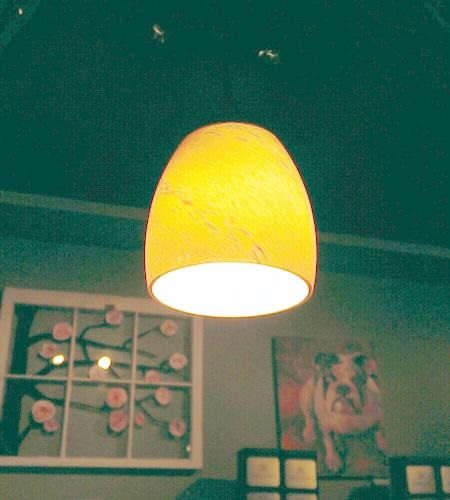
\includegraphics[width=7cm,height=9cm,keepaspectratio]{images/ch5/bulb_msr.jpg}
   		\caption{}
  	\end{subfigure}
  	\caption{a) Input Image b)Enhanced Image using MSR}
  	\label{fig:msr}
\end{figure}

Figure \ref{fig:msrcr} shows the original low light image of lamp and enhanced image using Multi-Scale Retinex with Color Restoration(MSRCR) . It is clear enhancement in Figure \ref{fig:msrcr}(b). The background objects of in figure \ref{fig:msrcr}(b) are more clear than original image. The Absolute Mean Difference(AMD),Root Mean Square and Entropy for Multi-Scale Retinex with Color Restoration((MSRCR) model of enhanced image of lamp is $67.0909,15.7330$ and $6.3657$ respectively      

\begin{figure}[!htb]
	\begin{subfigure}{8cm}
		\centering    
    	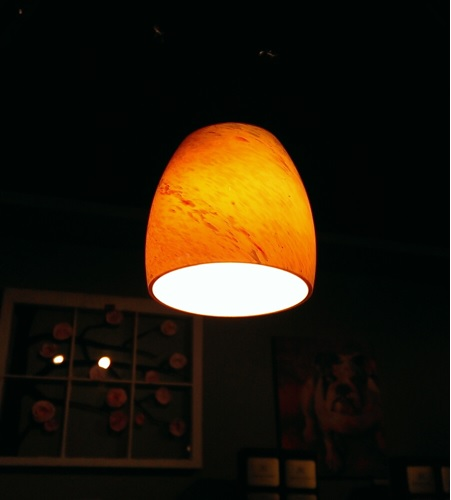
\includegraphics[width=7cm,height=9cm,keepaspectratio]{images/ch5/bulb_input.jpg}
    	\caption{} 
    \end{subfigure}
  	\begin{subfigure}{6cm}
  		\centering
  		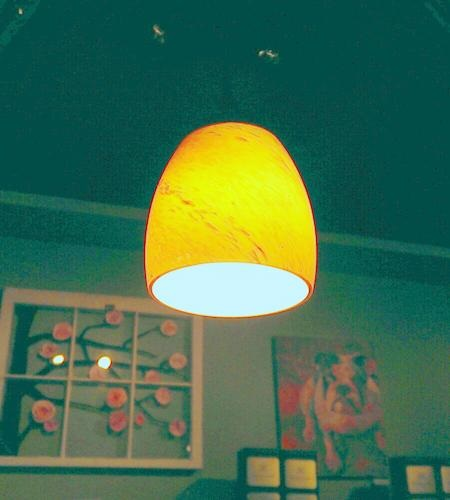
\includegraphics[width=7cm,height=9cm,keepaspectratio]{images/ch5/bulb_msrcr.jpg}
   		\caption{}
  	\end{subfigure}
  	\caption{a) Input Image b)Enhanced Image using MSRCR}
  	\label{fig:msrcr}
\end{figure}


Now consider second input image of palace. This image is also taken in low light and will test it for different Retinex Models. Figure \ref{fig:ssrPalace} shows the original low light image of palace and enhanced image using Single-Scale Retinex(SSR) model. In the original image (figure \ref{fig:ssrPalace} (a))  the palace,the valley, edges of rock,small bushy plants and lamps are not clear but these are very clear in the enhanced image(Figur \ref{fig:ssrPalace} (b)). The Absolute Mean Difference(AMD),Root Mean Square and Entropy for Single Scale Retinex(SSR) Model of enhanced image of palace is $103.9633,15.9031$ and $6.8944$ respectively      

\begin{figure}[!htb]
	\begin{subfigure}{8cm}
		\centering    
    	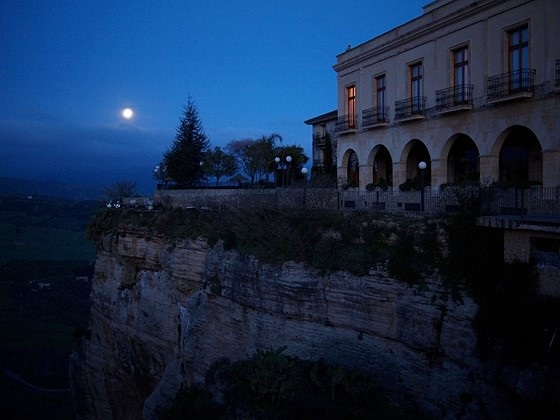
\includegraphics[width=7cm,height=9cm,keepaspectratio]{images/ch5/palace_input.jpg}
    	\caption{} 
    \end{subfigure}
  	\begin{subfigure}{6cm}
  		\centering
  		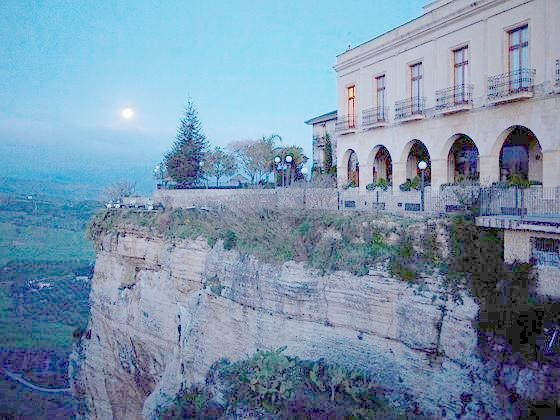
\includegraphics[width=7cm,height=9cm,keepaspectratio]{images/ch5/palace_ssr.jpg}
   		\caption{}
  	\end{subfigure}
  	\caption{a) Input Image b)Enhanced Image using SSR}
  	\label{fig:ssrPalace}
\end{figure}


%AMD_SSR =  103.9633
%r_SSR =  15.9031
%en_SSR =   6.8944
%AMD_MSR =  104.7167
%r_MSR =   15.9115
%en_MSR =    7.1499
%AMD_MSRCR =   92.2710
%r_MSRCR =   15.9138
%en_MSRCR =    7.7566

Figure \ref{fig:msrPalace} shows the original low light image of palace and enhanced image using Multi-Scale Retinex(MSR) model. In the original image (figure \ref{fig:msrPalace} (a))  the palace,the valley, edges of rock,small bushy plants and lamps are not clear but these are very clear in the enhanced image(Figure \ref{fig:msrPalace} (b)). The Absolute Mean Difference(AMD),Root Mean Square and Entropy for Multi Scale Retinex(MSR) Model of enhanced image of palace is $104.7167, 15.9115$ and $7.1499$ respectively      

\begin{figure}[!htb]
	\begin{subfigure}{8cm}
		\centering    
    	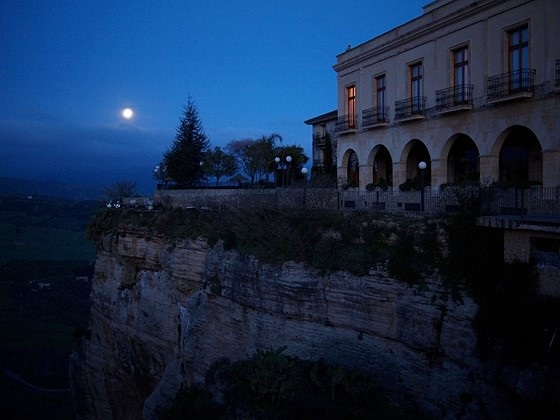
\includegraphics[width=7cm,height=9cm,keepaspectratio]{images/ch5/palace_input.jpg}
    	\caption{} 
    \end{subfigure}
  	\begin{subfigure}{6cm}
  		\centering
  		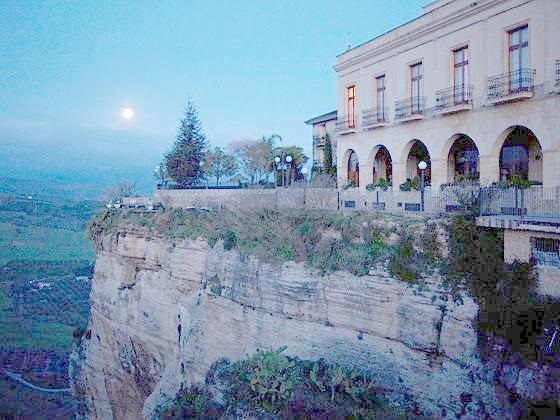
\includegraphics[width=7cm,height=9cm,keepaspectratio]{images/ch5/palace_msr.jpg}
   		\caption{}
  	\end{subfigure}
  	\caption{a) Input Image b)Enhanced Image using MSR}
  	\label{fig:msrPalace}
\end{figure}

Figure \ref{fig:msrcrPalace} shows the original low light image of palace and enhanced image using Multi-Scale Retinex with COlor Restoration(MSRCR) model. In the original image (figure \ref{fig:msrcrPalace} (a))  the palace,the valley, edges of rock,small bushy plants and lamps are not clear but these are very clear in the enhanced image(Figure \ref{fig:msrcrPalace} (b)). The Absolute Mean Difference(AMD),Root Mean Square and Entropy for Multi Scale Retinex with COlor Restoration(MSRCR) Model of enhanced image of palace is $92.2710, 15.9138$ and $7.7566$ respectively      

\begin{figure}[!htb]
	\begin{subfigure}{8cm}
		\centering    
    	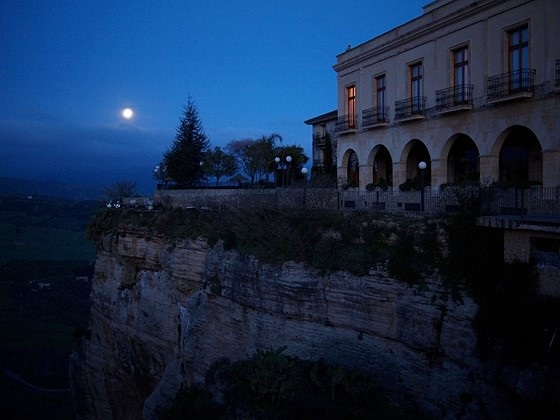
\includegraphics[width=7cm,height=9cm,keepaspectratio]{images/ch5/palace_input.jpg}
    	\caption{} 
    \end{subfigure}
  	\begin{subfigure}{6cm}
  		\centering
  		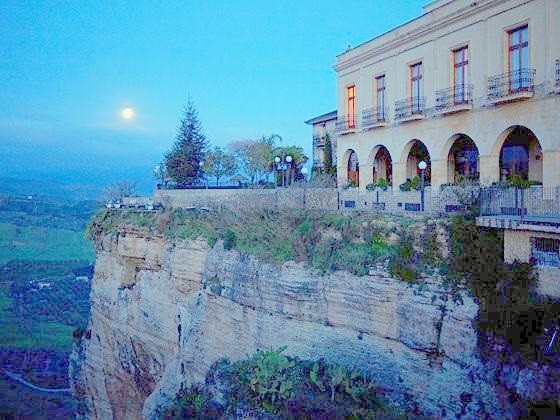
\includegraphics[width=7cm,height=9cm,keepaspectratio]{images/ch5/palace_msrcr.jpg}
   		\caption{}
  	\end{subfigure}
  	\caption{a) Input Image of Palace b)Enhanced Image of Palace using MSRCR}
  	\label{fig:msrcrPalace}
\end{figure}


Now consider third input image of robot. This image is also taken in low light and will test it for different Retinex Models. Figure \ref{fig:ssrRobot} shows the original low light image of robot and enhanced image using Single-Scale Retinex(SSR) model. In the original image of robot (figure \ref{fig:ssrRobot} (a))  the robot,laptop, laptop keypad and background strips are not clear but these are very clear in the enhanced image(Figur \ref{fig:ssrRobot} (b)). The Absolute Mean Difference(AMD),Root Mean Square and Entropy for Single Scale Retinex(SSR) Model of enhanced image of robot are $76.3404, 15.9245$ and $6.8248$ respectively      


\begin{figure}[!htb]
	\begin{subfigure}{8cm}
		\centering    
    	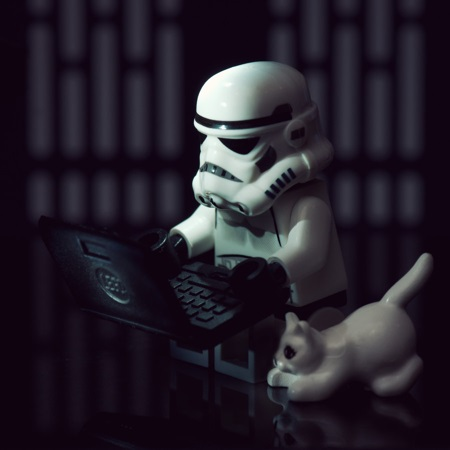
\includegraphics[width=7cm,height=9cm,keepaspectratio]{images/ch5/robot_input.jpg}
    	\caption{} 
    \end{subfigure}
  	\begin{subfigure}{6cm}
  		\centering
  		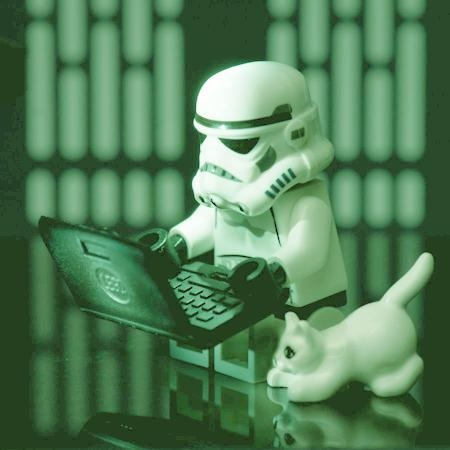
\includegraphics[width=7cm,height=9cm,keepaspectratio]{images/ch5/robot_ssr.jpg}
   		\caption{}
  	\end{subfigure}
  	\caption{a) Input Image of Robot b)Enhanced Image of Robot using SSR}
  	\label{fig:ssrRobot}
\end{figure}



%AMD_SSR =   76.3404
%r_SSR =   15.9245
%en_SSR =    6.8248
%AMD_MSR =   76.3157
%r_MSR =   15.9242
%en_MSR =    6.9686
%AMD_MSRCR =   74.7684
%r_MSRCR =   15.9179
%en_MSRCR =    7.0533
Figure \ref{fig:msrRobot} shows the original low light image of robot and enhanced image using Multi-Scale Retinex(MSR) model. In the original image of robot (figure \ref{fig:msrRobot} (a))  the robot,laptop, laptop keypad and background strips are not clear but these are very clear in the enhanced image(Figur \ref{fig:msrRobot} (b)). The Absolute Mean Difference(AMD),Root Mean Square and Entropy for Multi Scale Retinex(MSR) Model of enhanced image of robot are $76.3157, 15.9242$ and $6.9686$ respectively      


\begin{figure}[!htb]
	\begin{subfigure}{8cm}
		\centering    
    	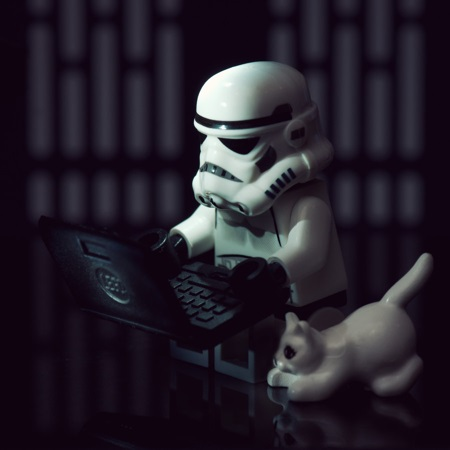
\includegraphics[width=7cm,height=9cm,keepaspectratio]{images/ch5/robot_input.jpg}
    	\caption{} 
    \end{subfigure}
  	\begin{subfigure}{6cm}
  		\centering
  		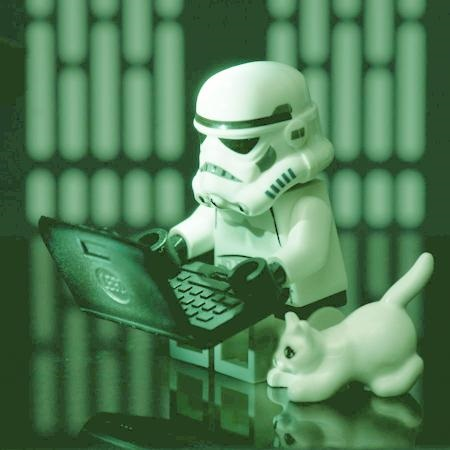
\includegraphics[width=7cm,height=9cm,keepaspectratio]{images/ch5/robot_msr.jpg}
   		\caption{}
  	\end{subfigure}
  	\caption{a) Input Image of Robot b)Enhanced Image of Robot using MSR}
  	\label{fig:msrRobot}
\end{figure}

Figure \ref{fig:msrcrRobot} shows the original low light image of robot and enhanced image using Multi-Scale Retinex with Color Restoration(MSRCR) model. In the original image of robot (figure \ref{fig:msrcrRobot} (a))  the robot,laptop, laptop keypad and background strips are not clear but these are very clear in the enhanced image(Figur \ref{fig:msrcrRobot} (b)). The Absolute Mean Difference(AMD),Root Mean Square and Entropy for Multi Scale Retinex with Color Restoration(MSRCR) Model of enhanced image of robot are $74.7684, 15.9179$ and $7.0533$ respectively      

\begin{figure}[!htb]
	\begin{subfigure}{8cm}
		\centering    
    	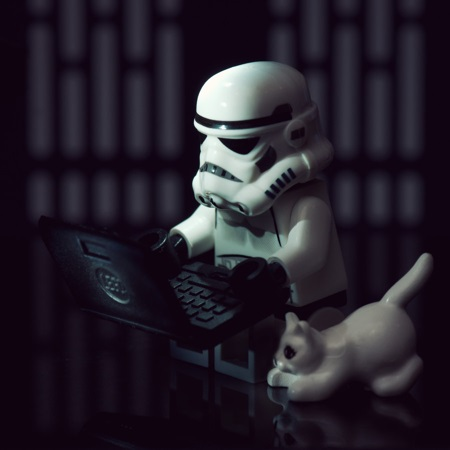
\includegraphics[width=7cm,height=9cm,keepaspectratio]{images/ch5/robot_input.jpg}
    	\caption{} 
    \end{subfigure}
  	\begin{subfigure}{6cm}
  		\centering
  		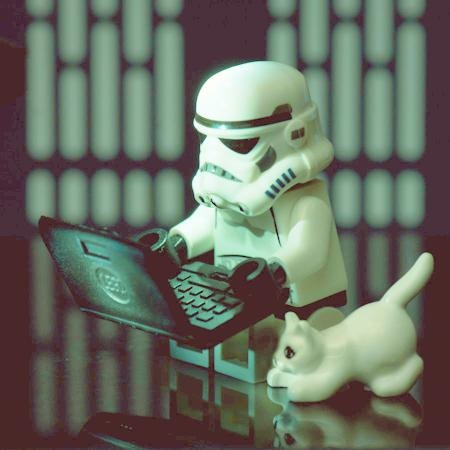
\includegraphics[width=7cm,height=9cm,keepaspectratio]{images/ch5/robot_msrcr.jpg}
   		\caption{}
  	\end{subfigure}
  	\caption{a) Input Image of Robot b)Enhanced Image of Robot using MSRCR}
  	\label{fig:msrcrRobot}
\end{figure}


\section{Power Law Transformation}
Now test above three images like bulb, palace and robot for Power Law Transformation. Figure \ref{fig:powerLaw} shows the original low light image of lamp and enhanced image using Power Law Transformation . It is clear enhancement in Figure \ref{fig:powerLaw}(b). The background objects of in figure \ref{fig:powerLaw}(b) are more clear than original image. The Absolute Mean Difference(AMD),Root Mean Square and Entropy for Power Law Transformation of enhanced image of lamp is $0.1068,0.1233$ and $5.2476$ respectively      


\begin{figure}[!htb]
	\begin{subfigure}{8cm}
		\centering    
    	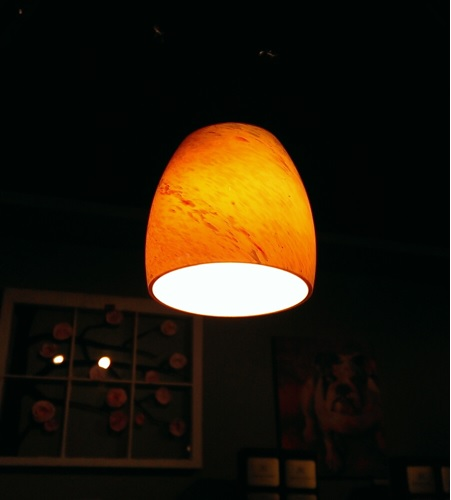
\includegraphics[width=7cm,height=9cm,keepaspectratio]{images/ch5/bulb_input.jpg}
    	\caption{} 
    \end{subfigure}
  	\begin{subfigure}{6cm}
  		\centering
  		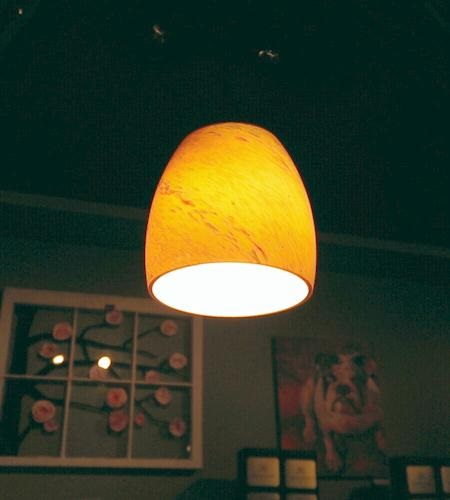
\includegraphics[width=7cm,height=9cm,keepaspectratio]{images/ch5/bulb_power.jpg}
   		\caption{}
  	\end{subfigure}
  	\caption{a) Input Image b)Enhanced Image using Power Law Transformation}
  	\label{fig:powerLaw}
\end{figure}

Figure \ref{fig:palacePowerLaw} shows the original low light image of palace and enhanced image using Power Law Transformation. In the original image of palace (figure \ref{fig:palacePowerLaw} (a))  the palace,the valley, edges of rock,small bushy plants and lamps are not clear but these are very clear in the enhanced image(Figure \ref{fig:palacePowerLaw} (b)). The Absolute Mean Difference(AMD),Root Mean Square and Entropy for Power Law Transformation of enhanced image of palace is $0.1857, 0.1957$ and $7.2592$ respectively      

%AMD_power =0.1857
%r_power =0.1957
%en_power =7.2592
\begin{figure}[!htb]
	\begin{subfigure}{8cm}
		\centering    
    	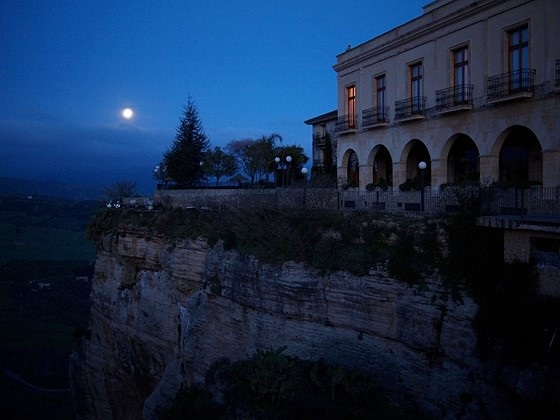
\includegraphics[width=7cm,height=9cm,keepaspectratio]{images/ch5/palace_input.jpg}
    	\caption{} 
    \end{subfigure}
  	\begin{subfigure}{6cm}
  		\centering
  		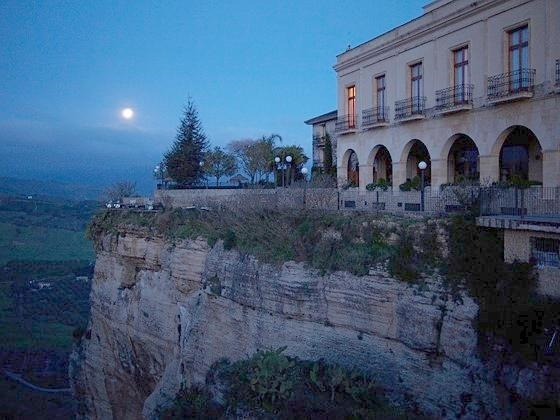
\includegraphics[width=7cm,height=9cm,keepaspectratio]{images/ch5/palace_power.jpg}
   		\caption{}
  	\end{subfigure}
  	\caption{a) Input Image of Palace b)Enhanced Image of palace using Power Law Transformation}
  	\label{fig:palacePowerLaw}
\end{figure}

Now consider third input image of robot. This image is also taken in low light and will test it for Power Law Transformation Figure \ref{fig:robotPowerLaw} shows the original low light image of robot and enhanced image using  Power Law Transformation. In the original image of robot (figure \ref{fig:robotPowerLaw} (a))  the robot,laptop, laptop keypad and background strips are not clear but these are very clear in the enhanced image(Figur \ref{fig:robotPowerLaw} (b)). The Absolute Mean Difference(AMD),Root Mean Square and Entropy for  Power Law Transformation of enhanced image of robot are $0.1953, 0.2010$ and $6.2899$ respectively      

%AMD_power =0.1953
%r_power =0.2010
%en_power =6.2899

\begin{figure}[!htb]
	\begin{subfigure}{8cm}
		\centering    
    	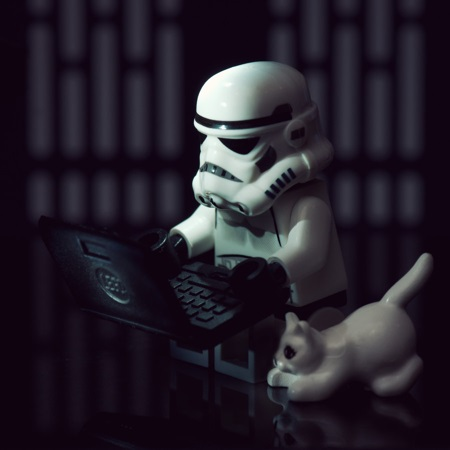
\includegraphics[width=7cm,height=9cm,keepaspectratio]{images/ch5/robot_input.jpg}
    	\caption{} 
    \end{subfigure}
  	\begin{subfigure}{6cm}
  		\centering
  		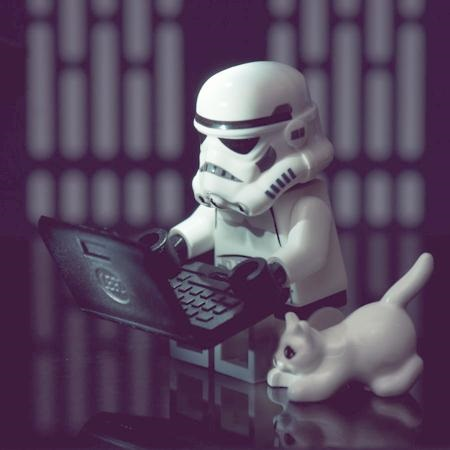
\includegraphics[width=7cm,height=9cm,keepaspectratio]{images/ch5/robot_power.jpg}
   		\caption{}
  	\end{subfigure}
  	\caption{a) Input Image of Robot b)Enhanced Image of Robot using Power Law Transformation}
  	\label{fig:robotPowerLaw}
\end{figure}


\section{Histogram Equalization}
Now test above same three images like bulb, palace and robot for Power Law Transformation. Figure \ref{fig:histEqu} shows the original low light image of lamp and enhanced image using Histogram Equalization. It is clear enhancement in Figure \ref{fig:histEqu}(b). The background objects of in figure \ref{fig:histEqu}(b) are more clear than original image. The Absolute Mean Difference(AMD),Root Mean Square and Entropy for Histogram Equalization of enhanced image of lamp is $104.7539,15.7363$ and $4.6140$ respectively      


\begin{figure}[!htb]
	\begin{subfigure}{8cm}
		\centering    
    	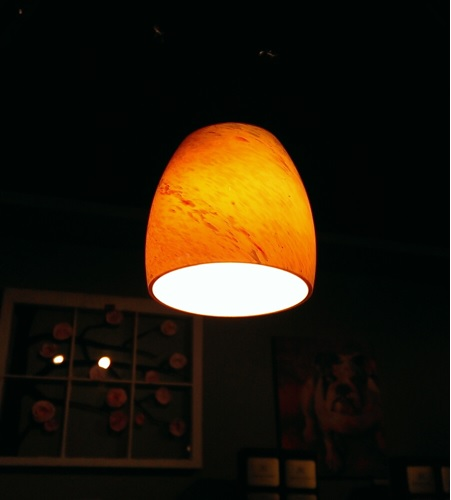
\includegraphics[width=7cm,height=9cm,keepaspectratio]{images/ch5/bulb_input.jpg}
    	\caption{} 
    \end{subfigure}
  	\begin{subfigure}{6cm}
  		\centering
  		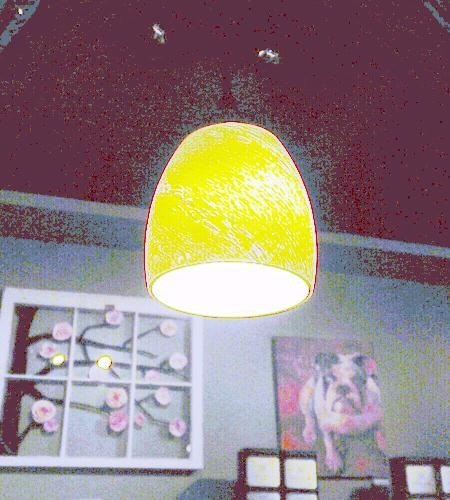
\includegraphics[width=7cm,height=9cm,keepaspectratio]{images/ch5/bulb_hist_equ.jpg}
   		\caption{}
  	\end{subfigure}
  	\caption{a) Input Image b)Enhanced Image using Histogram Equalization}
  	\label{fig:histEqu}
\end{figure}

Figure \ref{fig:palaceHistEq} shows the original low light image of palace and enhanced image using Histogram Equalization. In the original image of palace (figure \ref{fig:palaceHistEq} (a))  the palace,the valley, edges of rock,small bushy plants and lamps are not clear but these are very clear in the enhanced image(Figure \ref{fig:palaceHistEq} (b)). The Absolute Mean Difference(AMD),Root Mean Square and Entropy for Histogram Equalization of enhanced image of palace are $89.3506, 15.6912$ and $5.9325$ respectively      

%AMD_hist =89.3506
%r_hist =15.6912
%en_hist =5.9325

\begin{figure}[!htb]
	\begin{subfigure}{8cm}
		\centering    
    	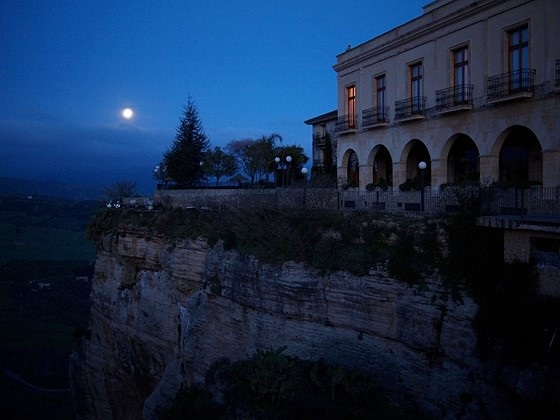
\includegraphics[width=7cm,height=9cm,keepaspectratio]{images/ch5/palace_input.jpg}
    	\caption{} 
    \end{subfigure}
  	\begin{subfigure}{6cm}
  		\centering
  		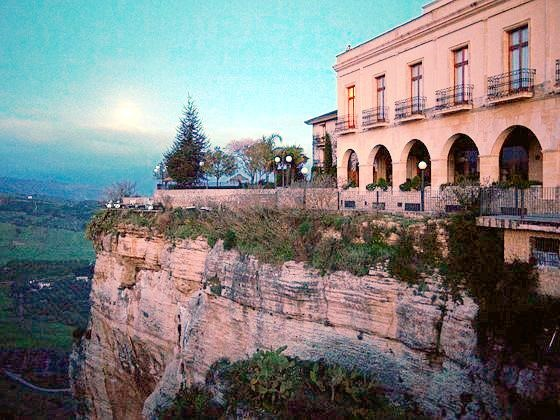
\includegraphics[width=7cm,height=9cm,keepaspectratio]{images/ch5/palace_hist_equ.jpg}
   		\caption{}
  	\end{subfigure}
  	\caption{a) Input Image of Palace b)Enhanced Image of palace using Histogram Equalization}
  	\label{fig:palaceHistEq}
\end{figure}

Now consider third input image of robot. This image is also taken in low light and will test it for Histogram Equalization Figure \ref{fig:robotHistEq} shows the original low light image of robot and enhanced image using  Histogram Equalization. In the original image of robot (figure \ref{fig:robotHistEq} (a))  the robot,laptop, laptop keypad and background strips are not clear but these are very clear in the enhanced image(Figur \ref{fig:robotHistEq} (b)). The Absolute Mean Difference(AMD),Root Mean Square and Entropy for  Histogram Equalization of enhanced image of robot are $93.1594, 15.1385$ and $5.5086$ respectively      

%AMD_hist =   93.1594
%r_hist =   15.1385
%en_hist =5.5086


\begin{figure}[!htb]
	\begin{subfigure}{8cm}
		\centering    
    	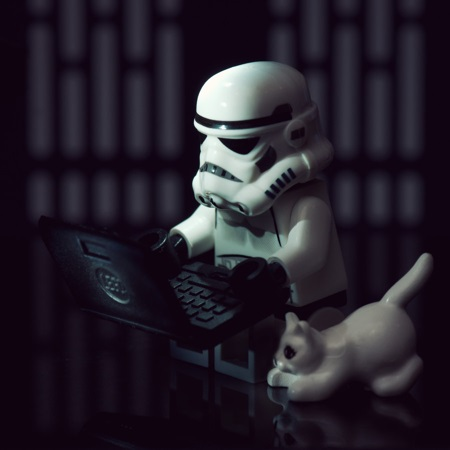
\includegraphics[width=7cm,height=9cm,keepaspectratio]{images/ch5/robot_input.jpg}
    	\caption{} 
    \end{subfigure}
  	\begin{subfigure}{6cm}
  		\centering
  		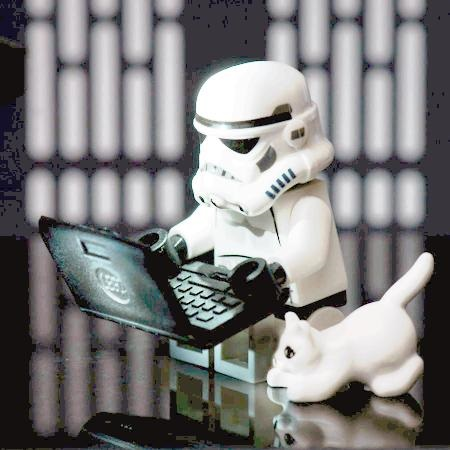
\includegraphics[width=7cm,height=9cm,keepaspectratio]{images/ch5/robot_hist_equ.jpg}
   		\caption{}
  	\end{subfigure}
  	\caption{a) Input Image of Robot b)Enhanced Image of Robot using Histogram Equalization}
  	\label{fig:robotHistEq}
\end{figure}



\section{Adaptive Histogram Equalization}
Now test same above three images like bulb, palace and robot for Power Law Transformation. Figure \ref{fig:AHE} shows the original low light image of lamp and enhanced image using Adaptive Histogram Equalization. It is clear enhancement in Figure \ref{fig:AHE}(b). The background objects of in figure \ref{fig:AHE}(b) are more clear than original image. The Absolute Mean Difference(AMD),Root Mean Square and Entropy for Adaptive Histogram Equalization of enhanced image of lamp is $12.9948,10.1784$ and $5.6053$ respectively      


\begin{figure}[!htb]
	\begin{subfigure}{8cm}
		\centering    
    	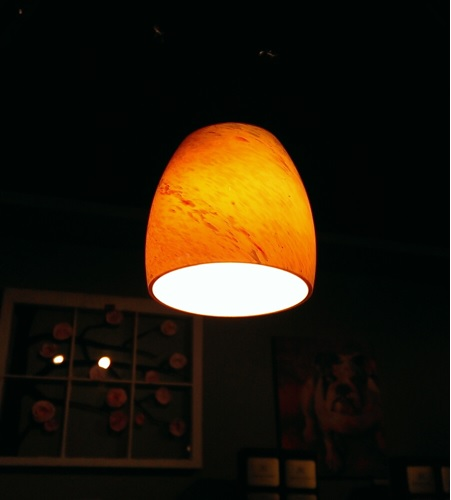
\includegraphics[width=7cm,height=9cm,keepaspectratio]{images/ch5/bulb_input.jpg}
    	\caption{} 
    \end{subfigure}
  	\begin{subfigure}{6cm}
  		\centering
  		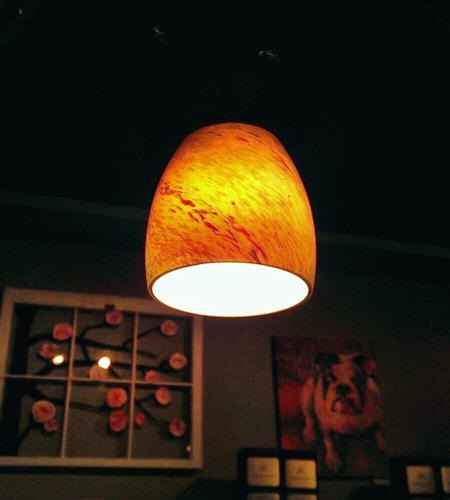
\includegraphics[width=7cm,height=9cm,keepaspectratio]{images/ch5/bulb_adapt_hist.jpg}
   		\caption{}
  	\end{subfigure}
  	\caption{a) Input Image b)Enhanced Image using Adaptive Histogram Equalization}
  	\label{fig:AHE}
\end{figure}


Figure \ref{fig:palaceAHE} shows the original low light image of palace and enhanced image using Adaptive Histogram Equalization. In the original image of palace (figure \ref{fig:palaceAHE} (a))  the palace,the valley, edges of rock,small bushy plants and lamps are not clear but these are very clear in the enhanced image(Figure \ref{fig:palaceAHE} (b)). The Absolute Mean Difference(AMD),Root Mean Square and Entropy for Adaptive Histogram Equalization of enhanced image of palace are $40.3042, 14.5370$ and $7.4680$ respectively      

%AMD_adaptive =   40.3042
%r_adaptive =   14.5370
%en_adaptive =7.4680

\begin{figure}[!htb]
	\begin{subfigure}{8cm}
		\centering    
    	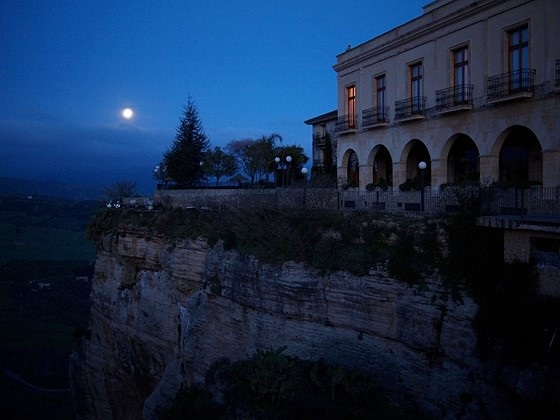
\includegraphics[width=7cm,height=9cm,keepaspectratio]{images/ch5/palace_input.jpg}
    	\caption{} 
    \end{subfigure}
  	\begin{subfigure}{6cm}
  		\centering
  		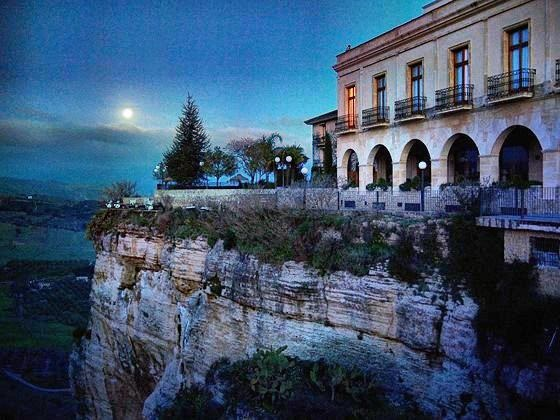
\includegraphics[width=7cm,height=9cm,keepaspectratio]{images/ch5/palace_adapt_hist.jpg}
   		\caption{}
  	\end{subfigure}
  	\caption{a) Input Image of Palace b)Enhanced Image of palace using Adaptive Histogram Equalization}
  	\label{fig:palaceAHE}
\end{figure}

Now consider third input image of robot. This image is also taken in low light and will test it for Adaptive Histogram Equalization Figure \ref{fig:robotAHE} shows the original low light image of robot and enhanced image using Adaptive Histogram Equalization. In the original image of robot (figure \ref{fig:robotAdaptive} (a))  the robot,laptop, laptop keypad and background strips are not clear but these are very clear in the enhanced image(Figure \ref{fig:robotAdaptive} (b)). The Absolute Mean Difference(AMD),Root Mean Square and Entropy for  Adaptive Histogram Equalization of enhanced image of robot are $30.0744, 12.6623$ and $7.2511$ respectively      

%AMD_adaptive =30.0744
%r_adaptive =12.6623
%en_adaptive =    7.2511


\begin{figure}[!htb]
	\begin{subfigure}{8cm}
		\centering    
    	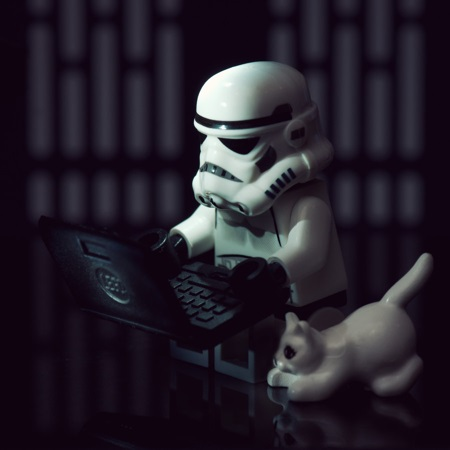
\includegraphics[width=7cm,height=9cm,keepaspectratio]{images/ch5/robot_input.jpg}
    	\caption{} 
    \end{subfigure}
  	\begin{subfigure}{6cm}
  		\centering
  		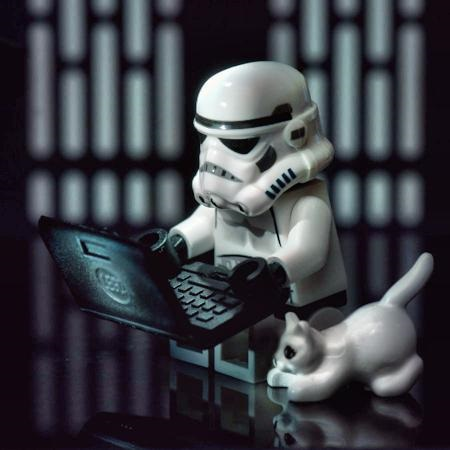
\includegraphics[width=7cm,height=9cm,keepaspectratio]{images/ch5/robot_adapt_hist.jpg}
   		\caption{}
  	\end{subfigure}
  	\caption{a) Input Image of Robot b)Enhanced Image of Robot using Adaptive Histogram Equalization}
  	\label{fig:robotAHE}
\end{figure}

Now compare these three images using different Retinex Models, Power Law Transformation, Histogram Equalization and Adaptive Histogram Equalization shown in table \ref{tab:lampTable},\ref{tab:palaceTable} and \ref{tab:robotTable} .

\begin{table}
	%\begin{center}
	\caption{Comparison for Lamp Image.}
    \label{tab:lampTable}
    \center
    \begin{tabular}{ |p{2cm}||p{2cm}|p{2cm}|p{2cm}|  }

 		\hline
	 	%\multirow{3}{*}{\rotatebox[origin=c]{90}{rota}
 		\multirow{2}{*}{\rotatebox[origin=c]{0}{Technique}}&\multicolumn{3}{|c|}{Lamp} \\
 		\cline{2-4}
  			&AMD&RMSE&Entropy    \\
 		\hline
 			SSR& 69.840  &15.7384 &4.9043 \\
 		\hline
 			MSR &69.9617 &15.7384 &5.0033  \\
 		\hline
 			MSRCR& 67.0909  &15.7330 &6.3657 \\
 		\hline
 			PLT& 0.1068  &0.1233 &5.2476\\
 		\hline
 			HE& 104.7539  &15.7363 &4.6140 \\
 		\hline
 			AHE& 12.9948  & 10.1784& 5.6053 \\
 		\hline
	\end{tabular}
\end{table}

%SSR\\
%AMD = 69.8401
%r = 15.7384
%en = 4.9043
%MSR\\
%AMD = 69.9617
%r = 15.7384
%en = 5.0033
%MSRCR\\
%AMD = 67.0909
%r = 15.7330
%en = 6.3657    
    
%Power Transformation\\
%AMD = 0.1068
%r = 0.1233
%en = 5.2476

%Histogram Equalization\\
%AMD = 104.7539
%r = 15.7363
%en = 4.6140

%Adaptive Histogram Equalization\\
%AMD = 12.9948
%r = 10.1784
%en = 5.6053


\begin{table}
	%\begin{center}
	\caption{Comparison for Palace Image.}
    \label{tab:palaceTable}
    \center
    \begin{tabular}{ |p{2cm}||p{2cm}|p{2cm}|p{2cm}|  }

 		\hline
	 	%\multirow{3}{*}{\rotatebox[origin=c]{90}{rota}
 		\multirow{2}{*}{\rotatebox[origin=c]{0}{Technique}}&\multicolumn{3}{|c|}{Lamp} \\
 		\cline{2-4}
  			&AMD&RMSE&Entropy    \\
 		\hline
 			SSR& 69.840  &15.7384 &4.9043 \\
 		\hline
 			MSR &69.9617 &15.7384 &5.0033  \\
 		\hline
 			MSRCR& 67.0909  &15.7330 &6.3657 \\
 		\hline
 			PLT& 0.1068  &0.1233 &5.2476\\
 		\hline
 			HE& 104.7539  &15.7363 &4.6140 \\
 		\hline
 			AHE& 12.9948  & 10.1784& 5.6053 \\
 		\hline
	\end{tabular}
\end{table}


\begin{table}
	%\begin{center}
	\caption{Comparison for Lamp Image.}
    \label{tab:robotTable}
    \center
    \begin{tabular}{ |p{2cm}||p{2cm}|p{2cm}|p{2cm}|  }

 		\hline
	 	%\multirow{3}{*}{\rotatebox[origin=c]{90}{rota}
 		\multirow{2}{*}{\rotatebox[origin=c]{0}{Technique}}&\multicolumn{3}{|c|}{Lamp} \\
 		\cline{2-4}
  			&AMD&RMSE&Entropy    \\
 		\hline
 			SSR& 69.840  &15.7384 &4.9043 \\
 		\hline
 			MSR &69.9617 &15.7384 &5.0033  \\
 		\hline
 			MSRCR& 67.0909  &15.7330 &6.3657 \\
 		\hline
 			PLT& 0.1068  &0.1233 &5.2476\\
 		\hline
 			HE& 104.7539  &15.7363 &4.6140 \\
 		\hline
 			AHE& 12.9948  & 10.1784& 5.6053 \\
 		\hline
	\end{tabular}
\end{table}
